\chapter{Implementasi dan Pengujian}
\label{chap:implementasiPengujian}

\section{Implementasi}
\label{sec:implementasi}

\subsection{Lingkungan Implementasi}
		\label{sec:lingkungan_implementasi}
			Implementasi perangkat lunak ini dilakukan di dua buah komputer. Implementasi pertama dilakukan pada komputer peneliti untuk keperluan pengujian fungsional. Komputer tersebut memiliki spesifikasi sebagai berikut:
				\begin{enumerate}
					\item Processor: 3.20Ghz 
					\item RAM: 4.00 GB DDR3	
					\item Sistem Operasi: Windows 8.1 Pro 64-bit 
					\item Versi Java: 1.8.0\_40
				\end{enumerate}
				Implementasi kedua dilakukan pada komputer server yang terhubung dengan jaringan FTIS untuk keperluan pengujian eksperimental. Komputer tersebut memiliki spesifikasi sebagai berikut:
				\begin{enumerate}
					\item Processor: 2.66Ghz 
					\item RAM: 4.00 GB DDR2	
					\item Sistem Operasi: Ubuntu server amd-64 
					\item Versi Java: 1.8.0\_66
				\end{enumerate}

\subsection{Hasil Implementasi}
				Hasil implementasi berupa aplikasi berbasis web terdiri dari lima halaman. 
				\textbf{Halaman \textit{Login}}\\
				Halaman \textit{login} digunakan pengguna untuk masuk ke dalam aplikasi. Pada halaman ini, pengguna dapat melakukan \textit{login} dengan mengisi \textit{email} pada kolom \textit{email} dan \textit{password} pada kolom \textit{password} kemudian mengklik tombol login. Tangkapan layar dari halaman \textit{login} dapat dilihat pada gambar \ref{fig:5_hasil_login}.
					\begin{figure}[H]
						\centering
						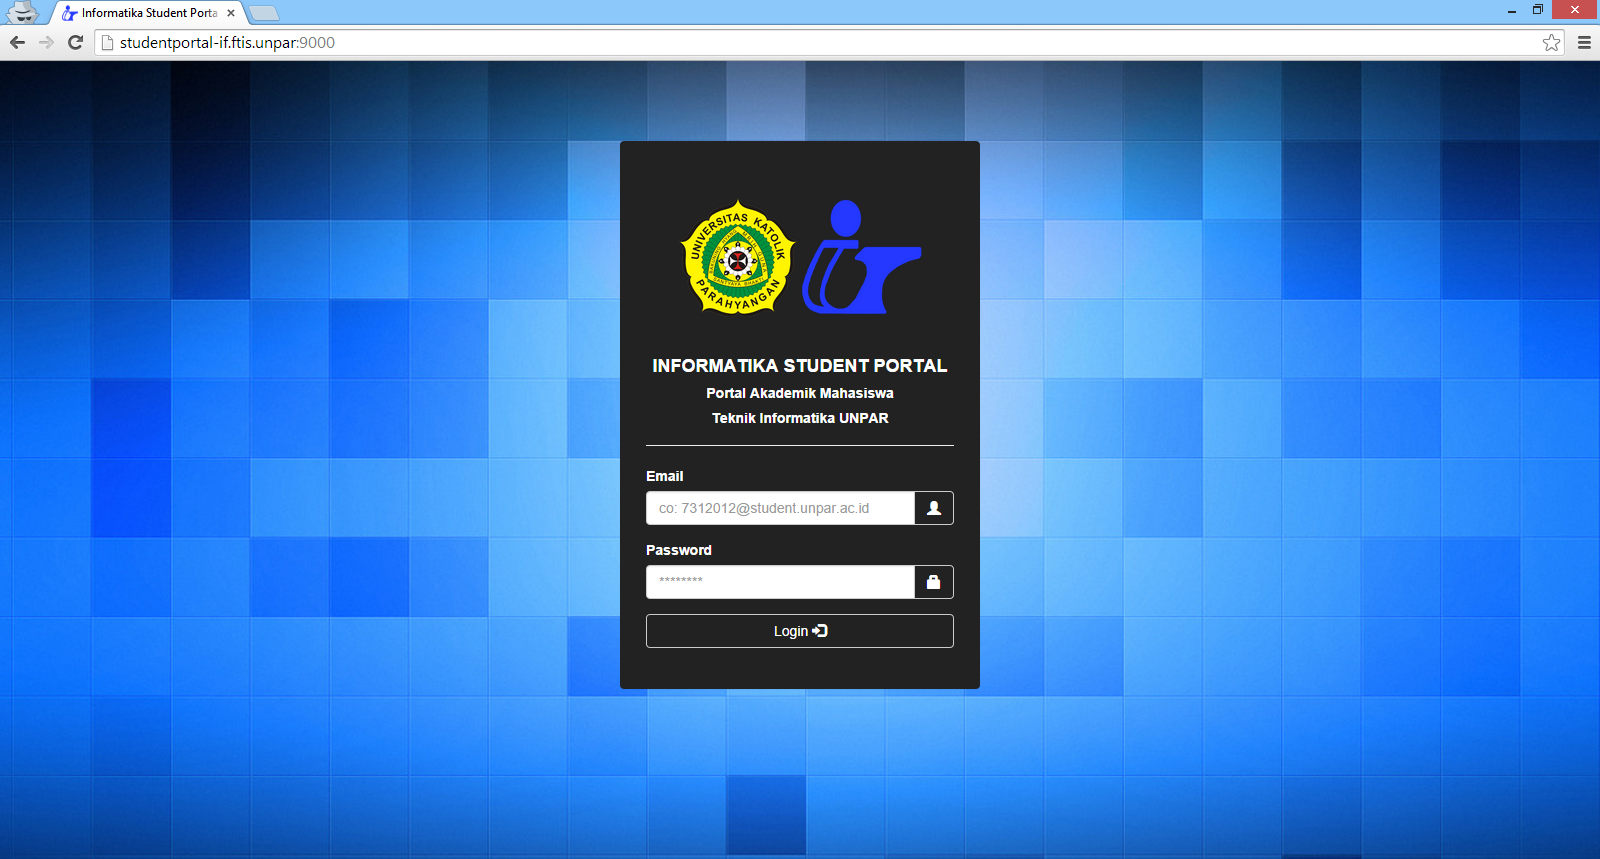
\includegraphics[scale=0.5]{Gambar/hasil_login}
						\caption{Halaman \textit{Login}} 
						\label{fig:5_hasil_login}
					\end{figure}
					
				\textbf{Halaman Utama}\\
				Halaman utama merupakan halaman yang pertama kali dituju setelah melakukan \textit{login}. Halaman utama menampilkan identitas pengguna dan \textit{link} menuju kode sumber aplikasi Informatika Student Portal. Pada halaman ini juga terdapat \textit{sidebar menu} yang diperoleh dari template StartBootstrap. Template tersebut juga digunakan pada halaman prasyarat mata kuliah, jadwal kuliah, dan data akademik. Tangkapan layar dari halaman utama dapat dilihat pada gambar \ref{fig:5_hasil_utama}.
					\begin{figure}[H]
						\centering
						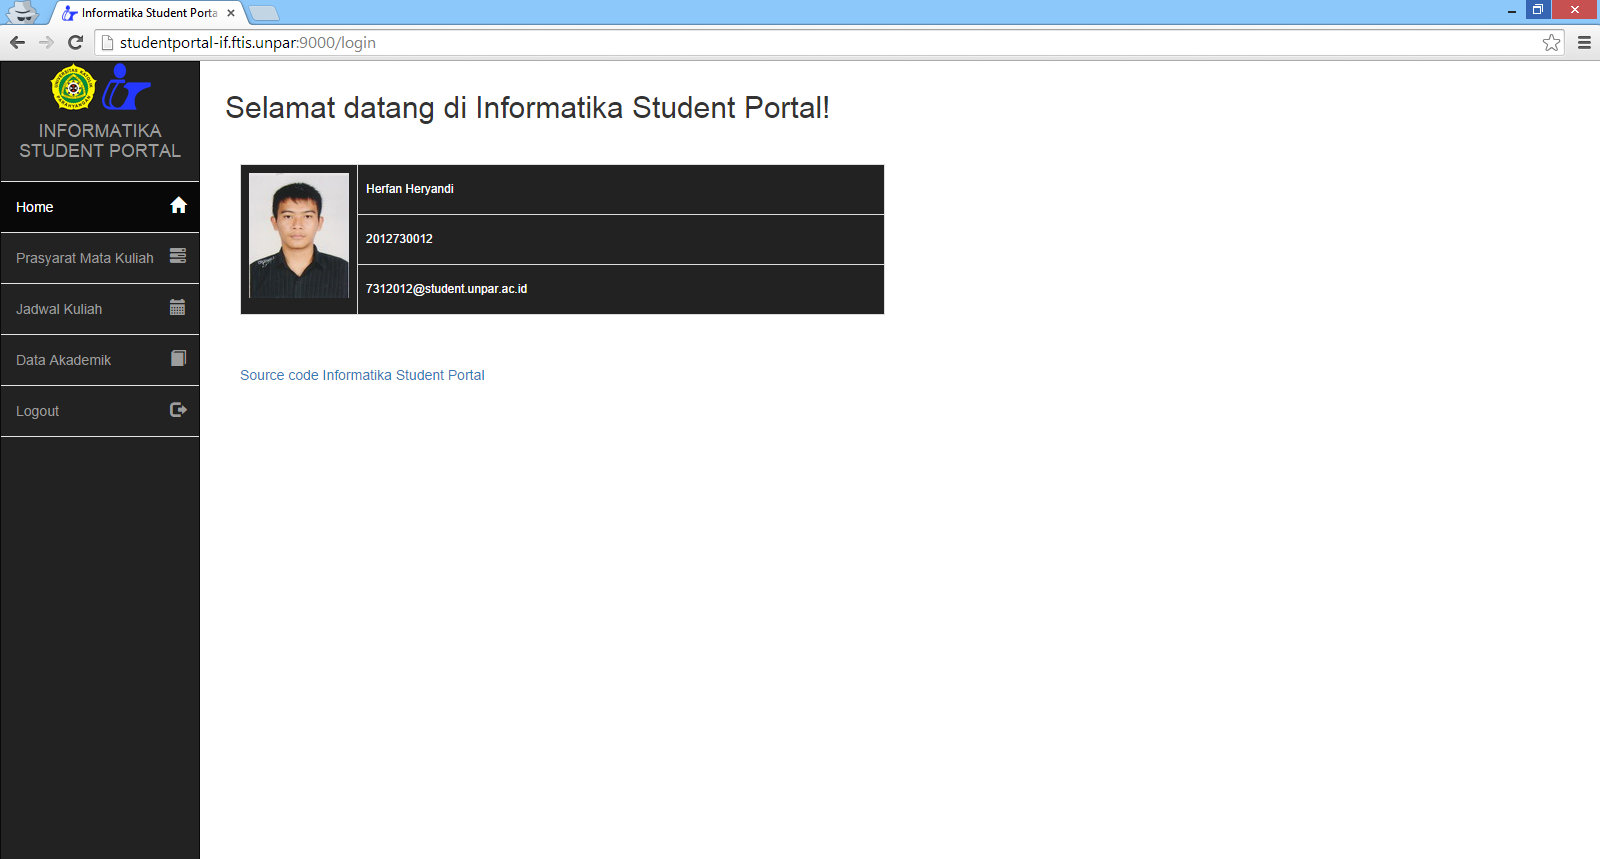
\includegraphics[scale=0.5]{Gambar/hasil_home}
						\caption{Halaman Utama} 
						\label{fig:5_hasil_utama}
					\end{figure}
						
				\textbf{Halaman Prasyarat Mata Kuliah}\\
				Halaman ini menampilkan tabel prasyarat mata kuliah. Jika prasyarat mata kuliah tersedia, pengguna dapat mengklik kode mata kuliah, kemudian akan diarahkan ke kode sumber aturan prasyarat mata kuliah tersebut. Tangkapan layar dari halaman prasyarat mata kuliah dapat dilihat pada gambar \ref{fig:5_hasil_prasyarat}.
					\begin{figure}[H]
						\centering
						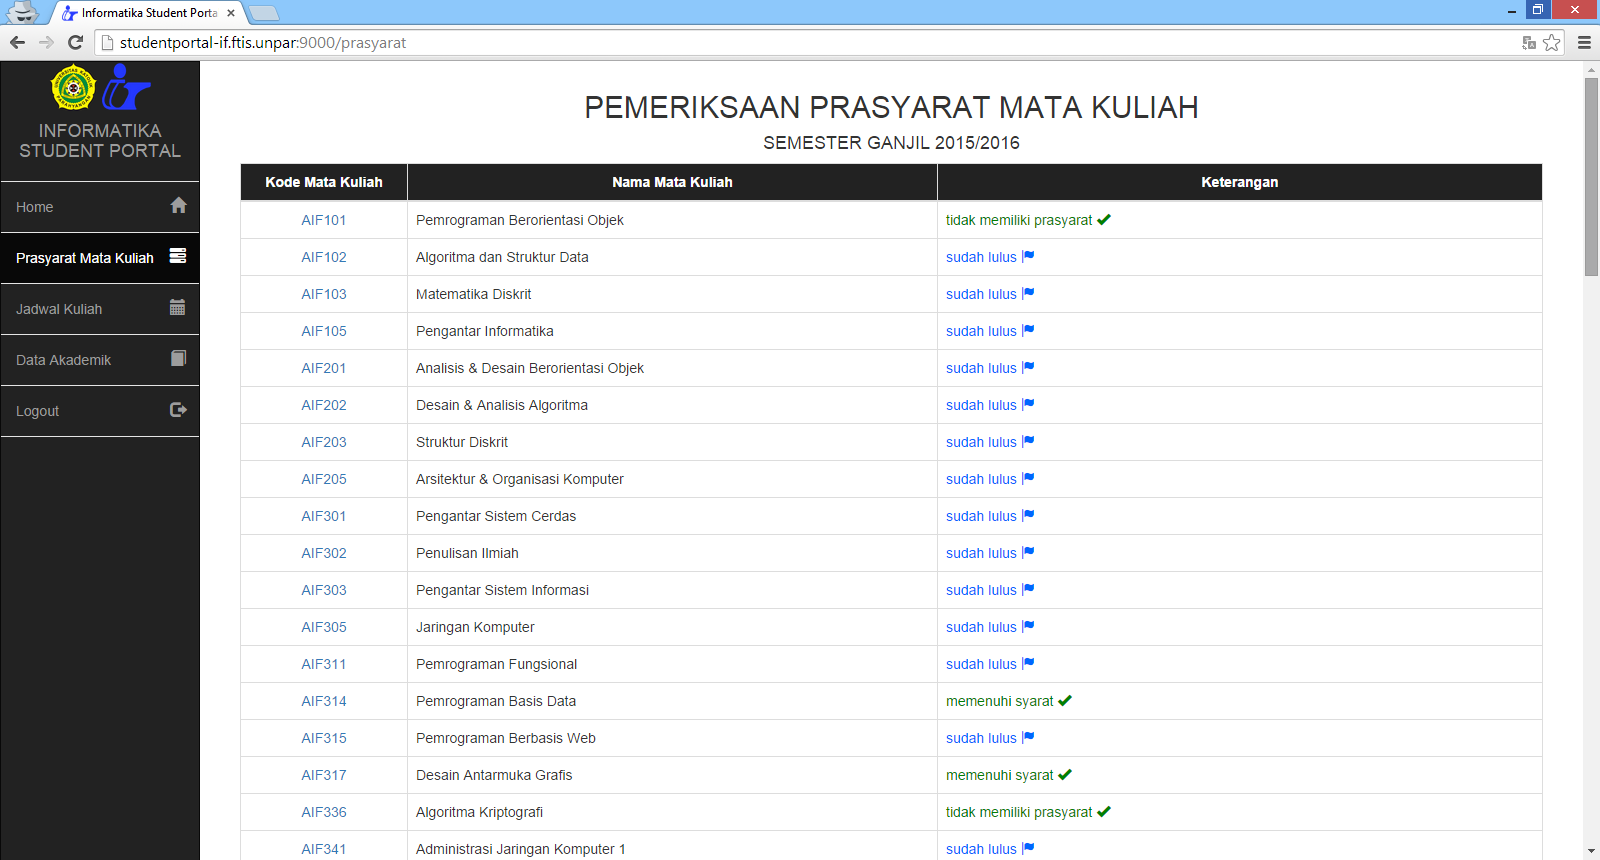
\includegraphics[scale=0.5]{Gambar/hasil_prasyarat}
						\caption{Halaman Prasyarat Mata Kuliah} 
						\label{fig:5_hasil_prasyarat}
					\end{figure}

				\textbf{Halaman Jadwal Kuliah}\\
				Halaman ini menampilkan jadwal kuliah yang tersusun dan terurut berdasarkan hari. Tangkapan layar dari halaman jadwal kuliah dapat dilihat pada gambar \ref{fig:5_hasil_jadwal}. Jika kode mata kuliah diklik, akan muncul \textit{popup} seperti pada gambar \ref{fig:5_hasil_rinci} yang berisi rincian dari jadwal kuliah tersebut.
				\begin{figure}[H]
						\centering
						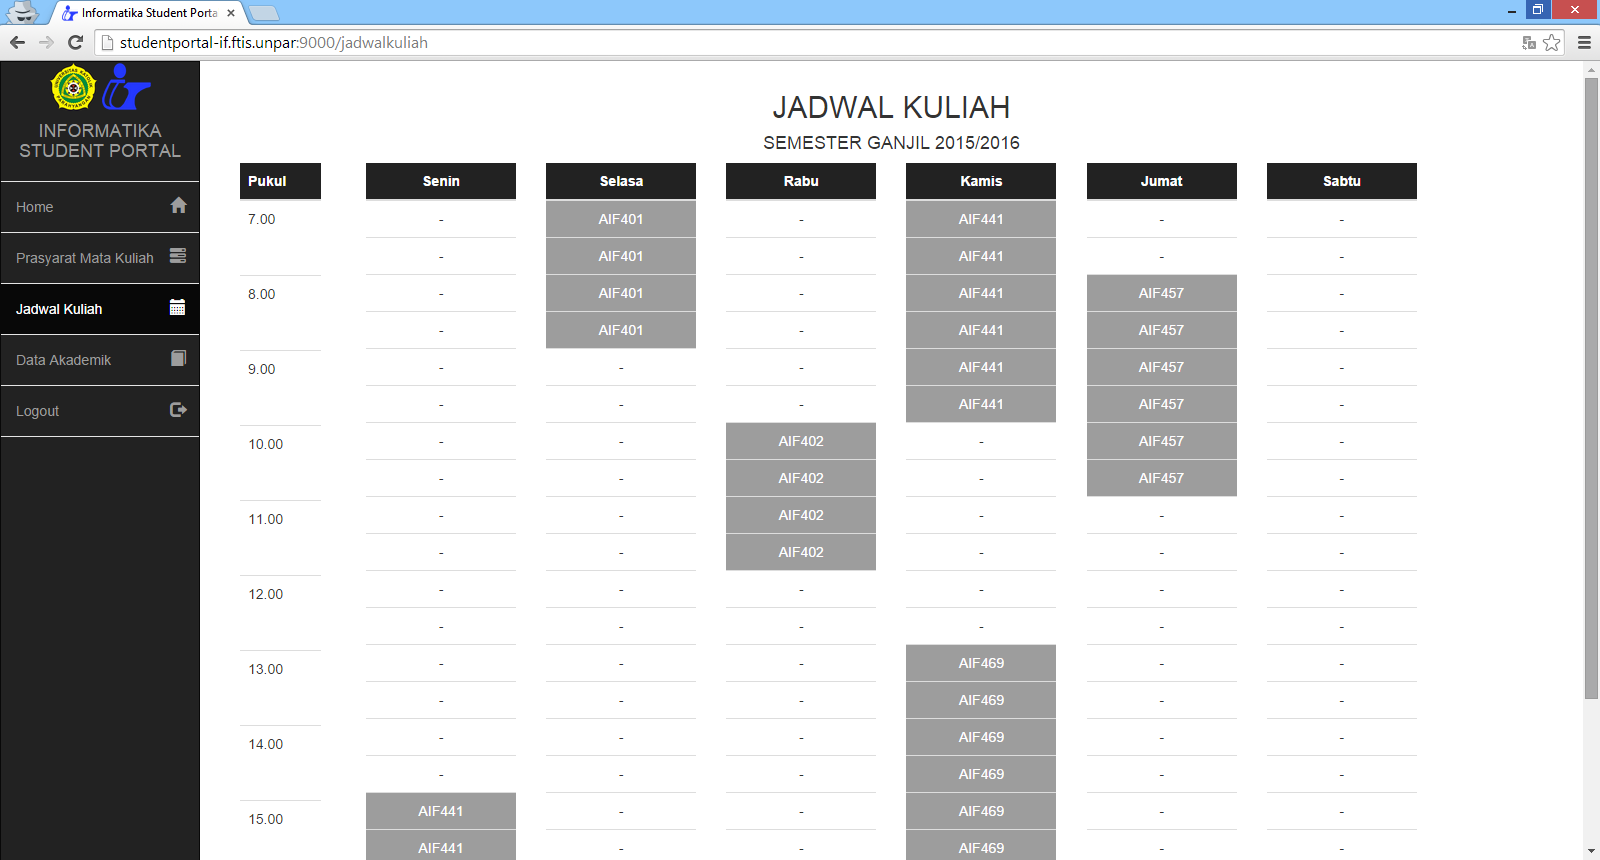
\includegraphics[scale=0.5]{Gambar/hasil_jadwal}
						\caption{Halaman Jadwal Kuliah} 
						\label{fig:5_hasil_jadwal}
					\end{figure}
					
					\begin{figure}[H]
						\centering
						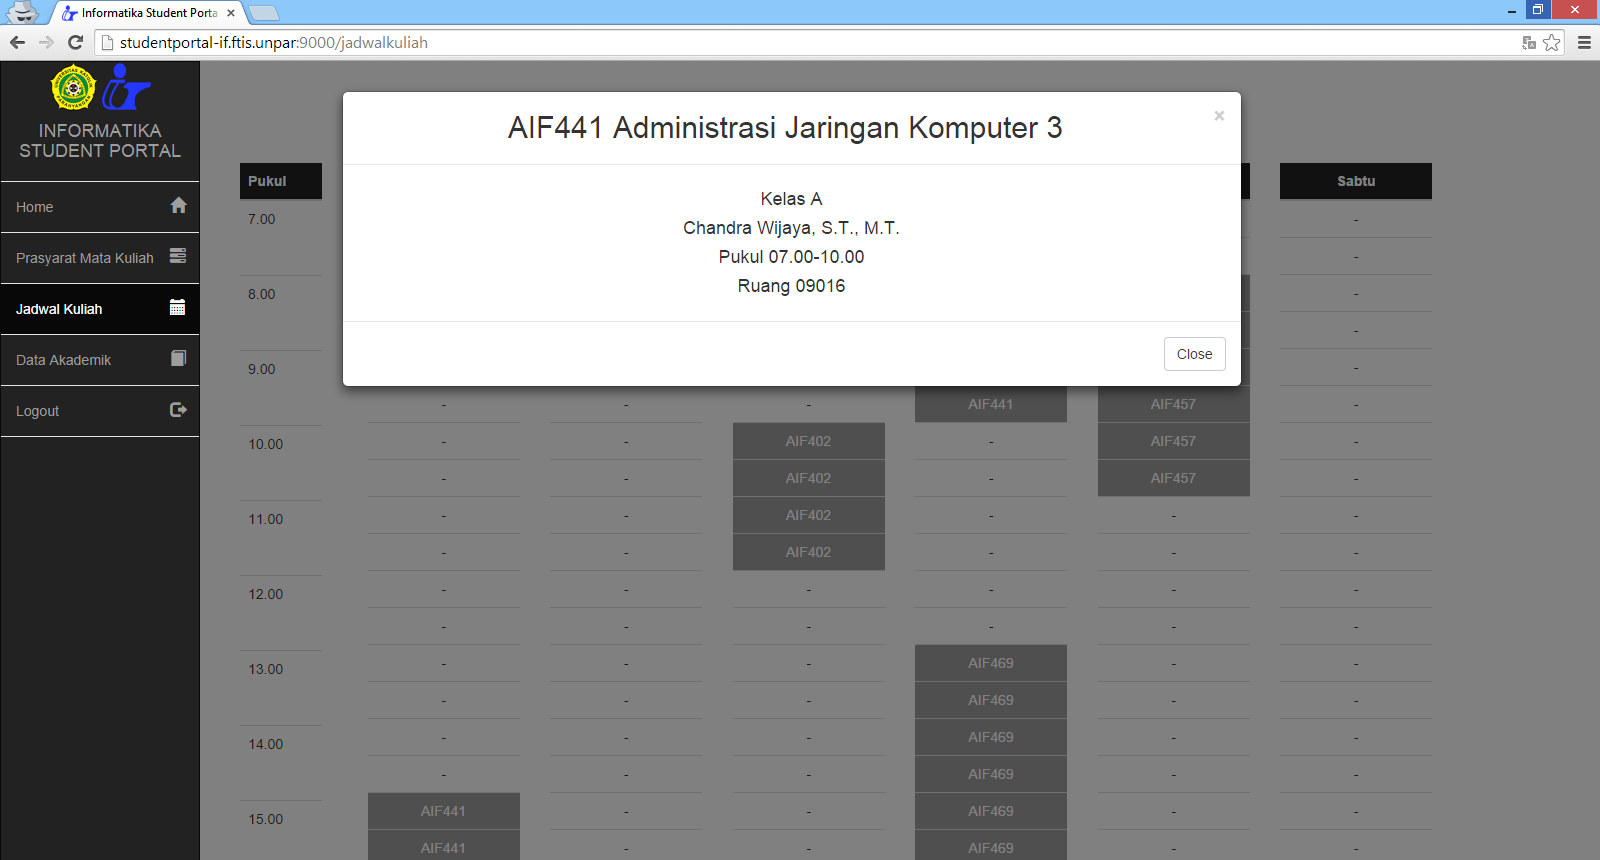
\includegraphics[scale=0.5]{Gambar/hasil_jadwal_popup}
						\caption{Rincian Jadwal Kuliah} 
						\label{fig:5_hasil_jadwal_rinci}
					\end{figure}
					
				\textbf{Halaman Data Akademik}\\
				Halaman ini menampilkan data akademik berupa IPS dan IPK yang langsung berubah ketika nilai sudah muncul, sisa SKS, dan status kelulusan mata kuliah pilihan wajib. Tangkapan layar dari halaman data akademik dapat dilihat pada gambar \ref{fig:5_hasil_ringkasan}.
				\begin{figure}[H]
						\centering
						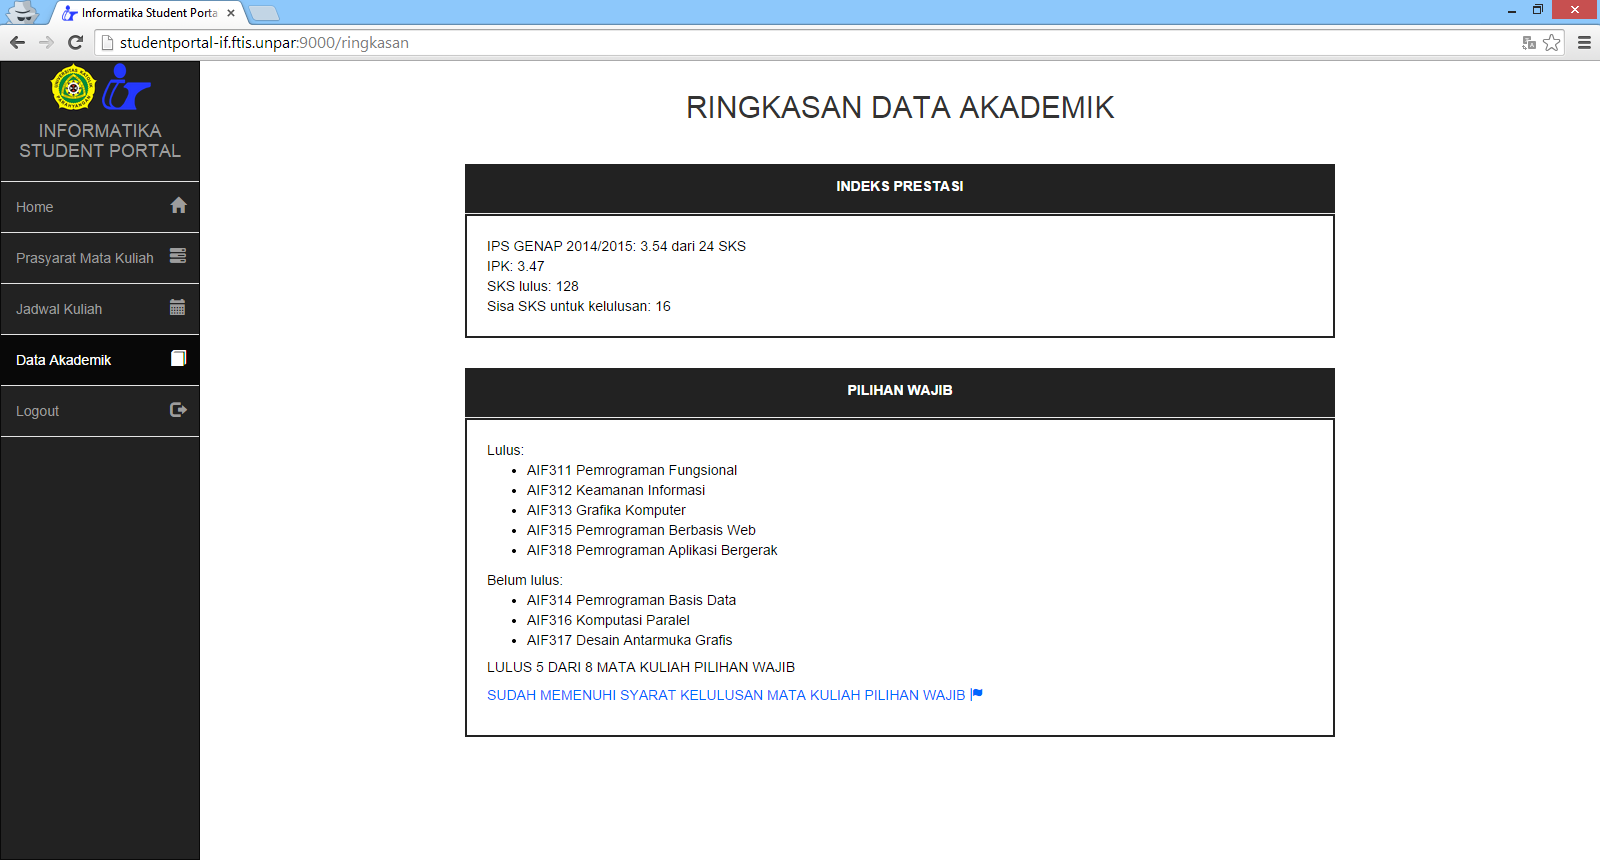
\includegraphics[scale=0.5]{Gambar/hasil_ringkasan}
						\caption{Halaman Data Akademik} 
						\label{fig:5_hasil_ringkasan}
					\end{figure}
				
\section{Pengujian}
			\subsection{Pengujian Fungsional} 
			Pengujian fungsional dilakukan untuk mengetahui kesesuaian reaksi perangkat lunak dengan reaksi yang diharapkan berdasarkan aksi pengguna terhadap perangkat lunak. Ada tujuh tes kasus yang diujikan, dan detail serta hasilnya dapat dilihat di tabel \ref{table:hasilFungsional}.
			
			\begin{table}[H]
			\centering
			\caption{Tabel Pengujian Fungsional}
				\begin{tabular}{|p{0.5cm}| p{3.5cm}| p{7cm}| p{2.25cm}|} \hline
				No.	&	Aksi Pengguna	&	Reaksi yang diharapkan	&	Reaksi Perangkat Lunak \\ \hline
				1.	&	Pengguna menjalankan aplikasi	&	Halaman \textit{login} akan ditampilkan	&	sesuai	\\ \hline
				2.	&	Pengguna memasukkan \textit{email} dan \textit{password}	&	Jika \textit{email} dan \textit{password}	sesuai, pengguna akan diarahkan ke halaman utama. & sesuai, namun foto profil tidak muncul jika belum validasi sertifikat SSL UNPAR\\ \hline
					&	&	Jika \textit{email} yang dimasukkan bukan \textit{email} \textit{student} UNPAR, akan ditampilkan pesan ``Email tidak valid''&	sesuai	\\ \hline
					&	&	Jika \textit{email} yang dimasukkan bukan \textit{email} mahasiswa teknik informatika, akan ditampilkan pesan ``Maaf, Anda bukan mahasiswa teknik informatika''	&	sesuai	\\ \hline
					&	&	Jika \textit{email} dan \textit{password} tidak sesuai atau mahasiswa bukan mahasiswa aktif, akan ditampilkan pesan ``Password yang Anda masukkan salah atau Anda bukan mahasiswa aktif''	&	sesuai	\\ \hline
				3.	&	Pengguna memilih menu ``Prasyarat Mata Kuliah'' &	Jika pengguna belum memiliki riwayat nilai(masih menempuh semester 1), akan ditampilkan pesan ``PRASYARAT BELUM TERSEDIA''	&	sesuai	\\ \hline
					&	&	Jika pengguna sudah memiliki riwayat nilai	akan ditampilkan tabel prasyarat mata kuliah beserta status pengambilannya &	sesuai	\\ \hline
				4.	&	Pengguna memilih menu ``Jadwal Kuliah'' &	Jika pengguna belum melakukan FRS, cuti studi, atau jadwal kuliah pengguna belum tersedia, akan ditampilkan pesan ``JADWAL KULIAH BELUM TERSEDIA''	&	sesuai	\\ \hline
					&	&	Jika jadwal kuliah pengguna sudah tersedia, akan ditampilkan jadwal kuliah dalam bentuk kalendar yang sudah diurutkan berdasarkan hari &	sesuai	\\ \hline
				5.	&	Pengguna memilih menu ``Data Akademik'' &	Jika pengguna belum memiliki riwayat nilai(masih menempuh semester 1), akan ditampilkan pesan ``DATA AKADEMIK BELUM TERSEDIA'' &	sesuai	\\ \hline
					&	&	Jika pengguna sudah memiliki riwayat nilai, akan ditampilkan ringkasan data akademik mahasiswa berupa IPS semester terakhir, IPK, SKS lulus, sisa SKS kelulusan, dan ringkasan data mengenai mata kuliah pilihan wajib &	sesuai	\\ \hline
				6.	&	Pengguna memilih tombol \textit{logout}	&	Pengguna akan diarahkan kembali ke halaman \textit{login} &	sesuai	\\ \hline
				7.	& Dua pengguna menggunakan aplikasi secara bersamaan	&	Pengguna dapat menggunakan aplikasi dengan akun yang sesuai &	sesuai	\\ \hline
				\end{tabular}
				\label{table:hasilFungsional}
			\end{table}
			
		\subsection{Pengujian Eksperimental} 
		Pengujian eksperimental dilakukan oleh mahasiswa angkatan 2012 sampai 2015.